\chapter{利用结构化信息的Twitter检索}
\label{IR}
%本章将进入论文排版的正文, 按元素分主要包括:
%{\kai 字体段落,图片表格,公式定理,参考文献}这几部分。
%这个样例文件将包括模板中使用到的所有格式、模板中自定义命令到或者特有的东西,
%都将被一一介绍,希望大家在排版自己的学位论文前能细致的看一遍,记住样例的格式和
%方法,方便上手。

\section{引言}
\label{sec:intro}
Twitter中的信息检索任务主要是给出关键词,然后在大量的tweet数据中找到与关键词话题相关的tweet。图\ref{Twitter_Search}是Twitter官方提供的检索主页,用户输入任何关键词,Twitter搜索引擎返回如图\ref{Twitter_SearchRes}的检索结果(Twitter中检索“sigir13”)。

\begin{figure}[htp]
\centering
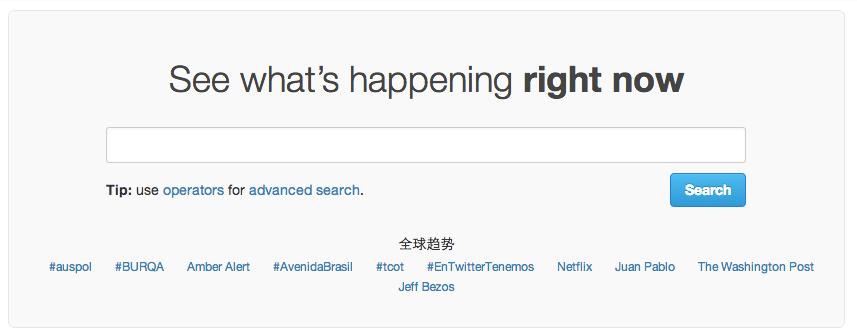
\includegraphics[height=170pt]{Twitter_Search.png}
\caption{Twitter检索主页}
\label{Twitter_Search}
\end{figure}

 \begin{figure}[htp]
\centering
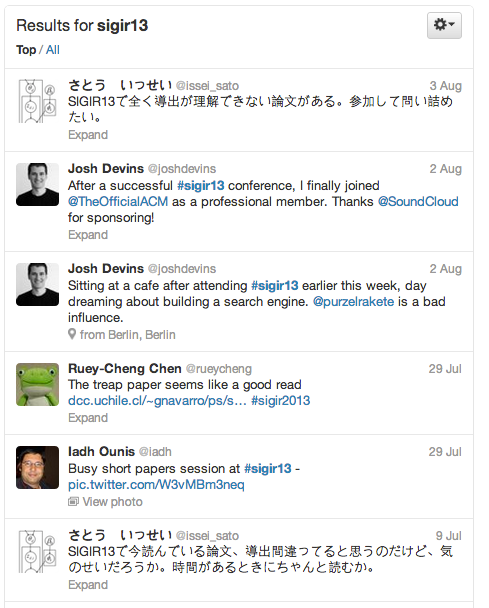
\includegraphics[height=350pt]{Twitter_SearchRes.png}
\caption{Twitter中检索sigir13返回结果}
\label{Twitter_SearchRes}
\end{figure}

目前传统的信息检索在Twitter中的应用主要还是度量关键词与tweet的话题相关性进行排序,另外辅助一些时间信息,如图\ref{Twitter_SearchRes}的返回结果就是在tweet与关键词在考虑话题相关程度的同时,按时间由近及远进行排序。但是Twitter是典型的社交媒体,每一个tweet都包含了丰富的社交媒体信息(如tweet作者的属性信息),这些信息并未得到足够的利用与开发,帮助Twitter中的信息检索。另外,传统Twitter中的信息检索都认为tweet的文本是短小非正式的噪音文本,不利于传统信息检索技术在Twitter中的应用。因此本章将研究如何利用tweet的文本信息和社交媒体信息帮助传统的Twitter信息检索。

现有Twitter上的信息检索方法简单的将每个tweet看成一个平面文本 \upcite{efron2010hashtag,duan2010empirical,massoudi2011incorporating,naveed2011searching},以前的工作表明,网页和普通的文本可以基于内容或结构划分成不重叠的小块,这些块和它们的组合信息可以被用来改进信息检索的效果\upcite{callan1994passage,ahnizeret2004information,fernandes2007computing}。虽然tweet是一个短文本,但是它也可以被看成是一个由多个块组合而成的文本。

图~\ref{TBB_examples}给出了一些由Yao Ming、BBC News和Lady Gaga发布的tweet样本\footnote{姚明是一位在NBA退役的中国职业篮球运动员, BBC News是英国广播公司的Twitter账户,Lady Gaga的是美国流行歌手。}。我们可以看到三者发布的tweet在文本结构上存在明显的差异:
  \begin{enumerate}
  \item Yao Ming发布的tweet仅仅是平面文本。
  \item BBC News发布的tweet都以链接结尾。
  \item Lady Gaga发布的tweet中包含大量的hashtag,链接和“@”符号。
  \end{enumerate}  

\begin{figure}[htp]
\centering
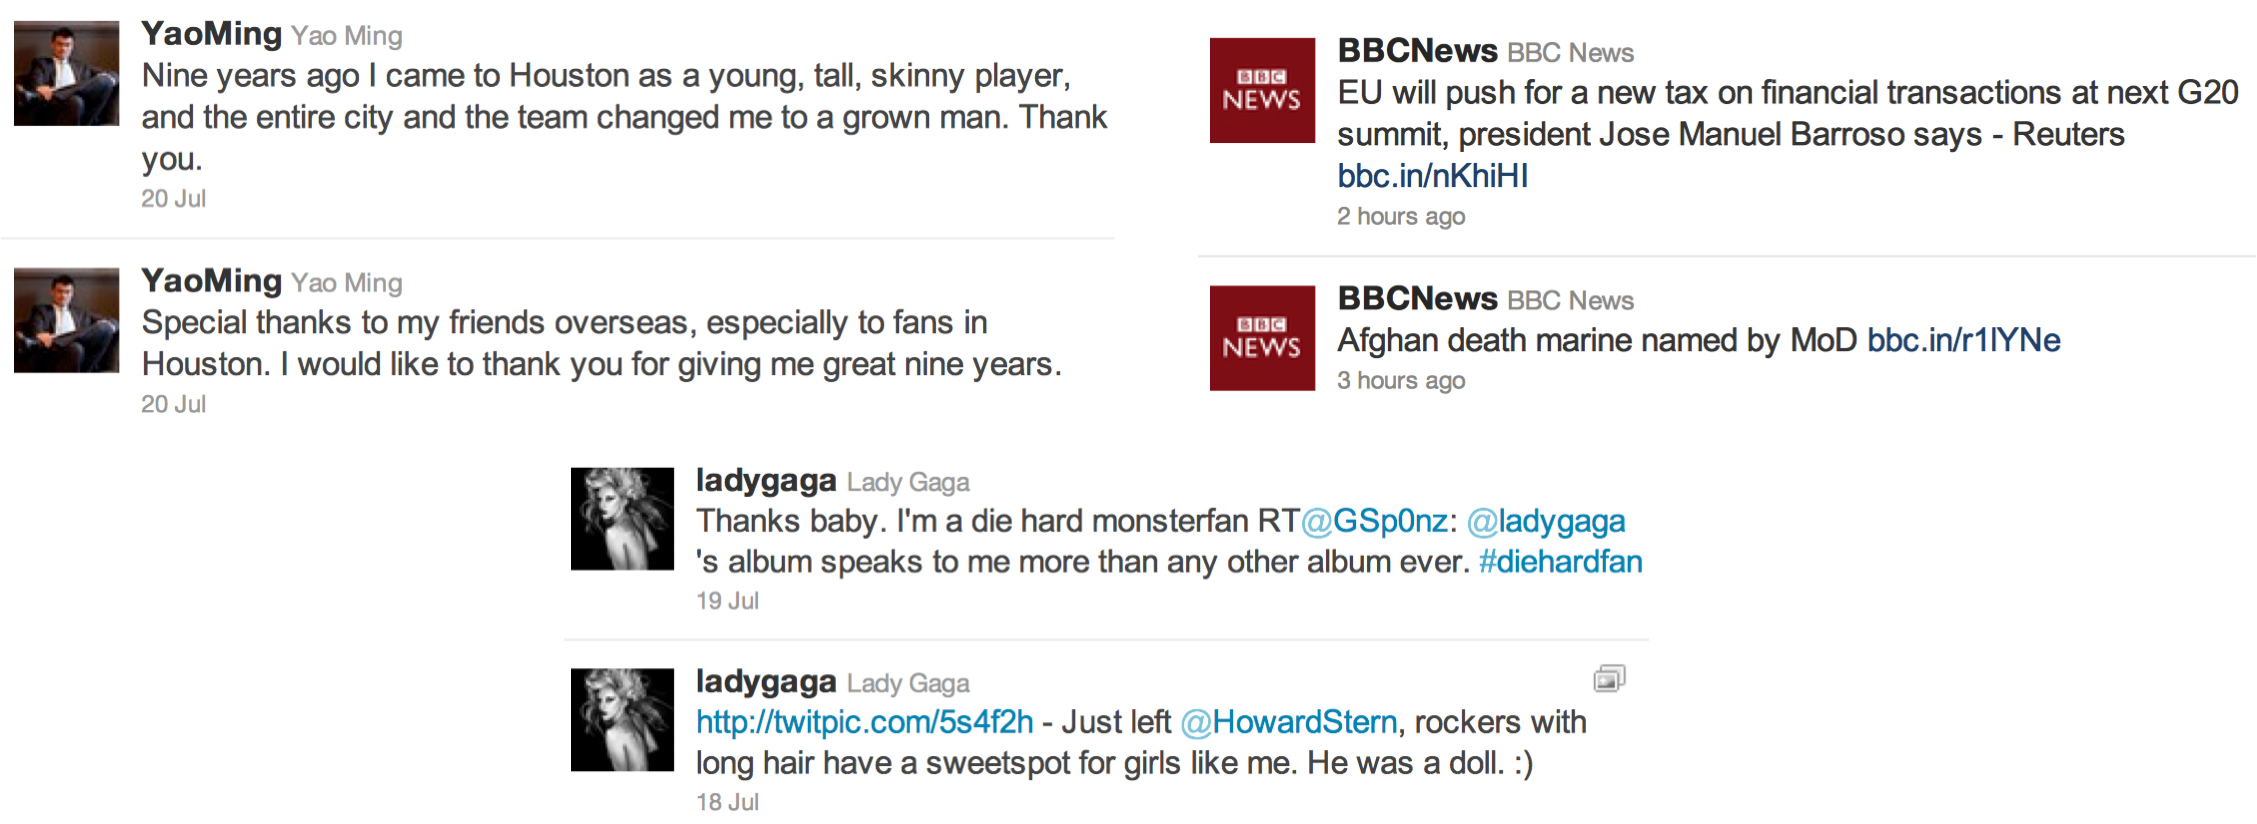
\includegraphics[height=150pt]{TBB_examples.png}
\caption{Yao Ming、BBC News和Lady Gaga的tweet样本示意图}
\label{TBB_examples}
\end{figure}

虽然平面文本、链接、hashtag和“@”符号的长度有差异,但我们都将其视为组成tweet的小块。利用这些小块,本章中我们将介绍一种从tweet文本中获取结构信息的方法,并以此来提高Twitter信息检索的效果。这种方法的动机主要是基于一个词在不同块中的出现往往存在着不同的排序权重。因为每个块都有自己本身的话题、功能、长度、位置、文本质量和语境等等。另外,tweet所对应块的序列组合结构也反映了tweet的话语转换信息以及质量信息。

我们将这种tweet中的块称为“Twitter积木 (Twitter Building Blocks或TBB)”,块的序列组合结构(TBB structures)则反映了tweet的结构信息。这些结构信息可以用来对tweet进行聚类,并且每个类别都有自身的属性。例如,与BBC News发布tweet结构相同的tweet(见图~\ref{TBB_examples})很有可能是新闻信息。另外,这种结构也与tweet文本的质量相关。因此,我们将开发这些结构信息并将其用到基于排序学习模型的Twitter信息检索方法中。

本章中,为了提高Twitter信息检索的效果,我们将设计一系列基于Twitter积木及其结构的特征。这些特征的主要优点在于它们不仅反映了tweet的结构信息而且信息的获取仅仅来自于tweet文本本身,并不依赖于其他社交媒体特征。我们将基于结构化信息的Twitter排序学习模型与目前最好的Twitter排序学习模型\upcite{duan2010empirical}进行了比较,实验结果表明仅仅只用我们设计的结构化特征开发的Twitter排序学习模型在tweet排序上可以达到最好的Twitter排序学习模型效果,而将社交媒体相关特征与结构化特征结合使用,tweet排序效果更好。

本章的主要工作如下:
  \begin{enumerate}
  \item 我们提出了Twitter积木的概念,Twitter积木是一种词串,它反映了各种交流信息,而Twitter积木各种序列组合则反映了tweet本身的话语转换。
  \item 我们设计了基于结构化信息的Twitter排序模型,并验证了该模型在对tweet排序上达到最好的Twitter排序模型效果,并且这种模型并未利用其他社交媒体特征。
  \item 我们将社交媒体特征与结构化特征相结合使用,获得了更好的Twitter信息检索效果。
  \end{enumerate}  

\section{相关工作}
\label{sec:rel}
我们从两个方面讨论相关工作:基于结构化的信息检索和Twitter信息检索。
\subsection{基于结构化的信息检索}
基于结构化的信息检索主要是利用结构化信息和文本的内容信息提高信息检索效果。这类方法的动机是基于同一个词在不同的文本块中拥有不同的排序权重,另外,文本块的特定组合结构也反映了特定的信息,这些信息可以被用于提高信息检索效果。Ahnizer等人利用手工设定块的权重来提高文本检索质量\upcite{ahnizeret2004information},它们利用不同块的不同权重综合计算不同词在排序当中的权重,以此改善排序效果。它们实验验证了这种方法有利于提高结构化文档的检索,特别是数据更新快的结构文档,例如,数字图书、论坛、新闻网站等。Fernandes和Moura等人提出了一种自动设定块权重的方法并以此提高网页检索的效果\upcite{fernandes2007computing,de2010using}。Cai等人也提出了一种利用切分网页获取结构化信息提高网页检索效果的方法\upcite{cai2004block}。以上方法都是基于同一词在不同块中存在不同的排序权重的思想。

\subsection{Twitter信息检索}
O'Connor等人开发了TweetMotif系统,主要用于Twitter中的话题发现及其摘要\upcite{o2010tweetmotif}。Efron提出了一种基于语言模型hashtag检索方法\upcite{efron2010hashtag},它利用检索到的hashtag对感兴趣的话题进行查询扩展,以此提高Twitter检索效果。Massoudi等人提出了一种基于tweet文本质量
的检索模型并取得了不错的检索效果\upcite{massoudi2011incorporating}。Naveed等人提出了一种Twitter检索方法,解决了tweet文本长度归一化与数据稀疏的问题\upcite{naveed2011searching}。但是以上的所有方法都并没有将tweet的结构化信息引入Twitter检索中。Duan等人提出了基于排序学习的Twitter检索方法\upcite{duan2010empirical},该方法不仅考虑了tweet内容的话题相关性,还考虑了tweet作者的权威性和tweet的其他特征。我们将此方法作为我们其中的一个基准系统进行比较,但是他们的方法依然没有考虑tweet文本的结构化信息。除了以上工作,最新的Twitter信息检索都没有考虑tweet文本的结构化信息\upcite{metzler2011usc,miyanishi2011trec,zhang2012query,darwish2012language,zhang2012transductive,miyanishi2013combining,choi2012quality,ferguson2012investigation,amati2012survival}。

绝大部分的Twitter 检索系统在构造检索模型时一般都认为tweet是一个平面文本,但是用户在编辑tweet时的一些习惯使得tweet文本呈现结构化的特点,以往通过开发文本的结构
信息能够帮助结构化文本的检索(例如,网页检索),因此我们希望利用tweet的文本结构信息帮助Twitter检索。我们首先定义Twitter积木以此捕获tweet文本结构,然后构造了Twitter积木自动识别器,通过对tweet积木的自动识别开发特征,设计了基于结构化信息的Twitter排序模型,最后实验验证该模型对于Twitter信息检索的有效性。

\section{Twitter积木(TBB)}
这一节我们主要介绍Twitter积木以及积木的自动识别。通过Twitter积木可以定义tweet的文本结构,这种结构反映了tweet的文本属性(如话语转换和文本质量)和潜在的社会属性。我们希望通过tweet文本的结构信息开发特征,帮助Twitter信息检索任务。

一个tweet可以看成由一些文本块组合而成的文本,而文本块则是一些词的排列组合而成。我们将这些文本块称为“Twitter积木(Twitter Building Blocks或TBB)”。各种Twitter积木的排列组合则构成了“Twitter积木结构(TBB structure)”。

\subsection{Twitter积木的定义}
在Twitter中人们经常使用三种方式表现其行为,包括标注(为tweet添加标签指明tweet的主题)、提及(在tweet中提及某人)、转发(再次重新发布其他人发布的tweet)。另外,tweet本身的内容也可以分成三类,包括链接、观点、普通文本。基于此我们定义了六种不同的Twitter积木:
  \begin{enumerate}
  \item {\bf 标签积木(TAG)}:“\#”和关键词的绑定使用,主要用来指明tweet的主题,如“\emph{\#iphone}”。
  \item {\bf 提及积木(MET)}:在tweet中提及某人的符合串,可以让对方看到此tweet,如“\emph{@ladygaga}”。
  \item {\bf 转发积木(RWT)}:指明复制或再次传播其他人发布tweet的符合串,如“\emph{RT @ladygaga}”。
  \item {\bf 链接积木(URL)}:链接到tweet本身内容以外的网址,如“\emph{http://www.facebook.com}”。
  \item {\bf 观点积木(COM)}:用来表达作者对其他Twitter积木的态度、评估、情绪。
  \item {\bf 普通文本积木(MSG)}:其他文本。
  \end{enumerate}  

图~\ref{TBB_gold}给出了手工标注Twitter积木的两个tweet样例。每个由下划线标注的词序列是一个Twitter积木。从图~\ref{TBB_gold}中我们看到 Tweet (a)是一个由“COM RWT MET MSG”积木结构组成的tweet,Tweet (b)则是由“MSG URL TAG”积木结构组成的tweet。积木本身的内容和组合反映了tweet的话语转换信息。例如,Tweet (a)是作者转发(RWT)用户@miiisha\_x的普通文本积木(MSG),这个普通文本积木(MSG)提及了(MET)用户@XPerkins,同时作者还给出了对于普通文本积木(MSG)的观点(COM)。Tweet (b)中作者则先后给出了普通文本积木(MSG)、一个链接积木(URL)和两个hashtag组成的标签积木(TAG),作者在后面两个积木提供了其他资源且标注了tweet的主题,使得其他读者能更好地理解原来普通文本积木(MSG)的内容。
\begin{figure}[htp]
\centering
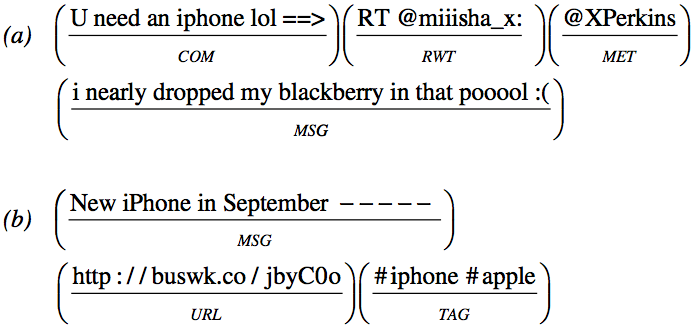
\includegraphics[height=150pt]{TBB_gold.png}
\caption{手工标注Twitter积木的tweet示意图}
\label{TBB_gold}
\end{figure}

为了理解人们是如何使用这些Twitter积木,我们随机的选择了2000个英文tweet\footnote{我们使用语言识别工具对非英语tweet进行过滤 \url{http://code.google.com/p/language-detection/}},并对其进行了Twitter积木及其结构的手工标注。在标注之前我们首先使用了O'Connor等人开发的工具\footnote{下载地址为:\url{https://github.com/brendano/tweetmotif}}自动地对每个tweet进行单词化(tokenized)\upcite{o2010tweetmotif}。表~\ref{TBB_Distr}给出了不同Twitter积木结构的比例分布。这里列出14个最常用的Twitter积木结构,其他非常用的Twitter积木结构则统称为“OTHERS”。我们可以看出“MSG”结构比例最高,这说明这种最简单的结构是最常用的Twitter积木结构。其他比例较高的Twitter积木结构是比较简单的,一般不超过三块积木。而由其他比例较低Twitter积木结构归类而成的“OTHERS”仅仅存在13\%,以上说明人们大多使用简单和固定的结构发布tweet。

\begin{table}[htp]
\centering
\caption{Twitter积木结构比例分布}
\label{TBB_Distr}
\begin{tabular}{|l |c|l |c|}
\hline
\textbf{Twitter积木类型} &\textbf{比例(\%)}&\textbf{Twitter积木类型} &\textbf{比例(\%)}\\
\hline
MSG & 30.25&TAG MSG & 1.55\\
MET MSG & 20.70&TAG MSG URL & 1.20\\
MSG URL & 18.40&RWT MSG URL & 0.95\\
OTHERS & 13.20&COM RWT MSG & 0.85\\
COM URL & 4.10&MET MSG URL & 0.85\\
MSG TAG & 2.65&MSG MET MSG & 0.70\\
MSG URL TAG & 2.10&RWT MSG TAG & 0.70\\
RWT MSG & 1.75&&\\
\hline
\end{tabular}
\end{table}

\subsection{Twitter积木自动标注}
手工标注每个tweet的Twitter积木及其结构显然是不可行的,因此我们设计了自动标注器来完成Twitter积木自动标注的任务。这个任务可以看成由两个子任务组成:Twitter积木的分类和Twitter积木的边界识别。这个任务十分类似于自然语言处理中的命名体识别问题(Named Entity Recognition)\upcite{tjong2003introduction},因此我们采用序列标注的方法(Sequential Labeling Approach)一同解决Twitter积木自动标注的两个子任务,另外,我们还采用了IOB-类型标注模式\upcite{ritter2011named,liu2011recognizing}。

输入一个tweet,我们的目的是输出一个序列Twitter积木块\emph{B$_1$B$_2$...B$_m$},其中\emph{B$_i$}是一个词串\emph{t$_{i1}$t$_{i2}$...t$_{in}$}。每一个在tweet中的词\emph{t$_{ij}$}将被标注一个标签\emph{“X\_Y” (X = \mbox{TAG,MET,RWT,URL,COM,MSG};Y = \mbox{B,I)}},这个标签说明了词的类型和是否是边界词。每个在同一个积木块中的词具有相同的 \emph{X}值,\emph{“Y = B”}表示词\emph{t$_{ij}$ (j=1)}为边界词,而 \emph{“Y = I”}表示为非边界词。例如,图~\ref{TBB_gold}中 Tweet (b)的词“iPhone” 和“\#iphone”,它们的标签分别是“MSG\_I”和“TAG\_B”。 

我们利用条件随机场(\emph{Conditional Random Field})进行序列标注\upcite{lafferty2001conditional},这种方法能够将设计的局部特征很好的纳入学习模型中。我们利用Twitter不同积木经常出现的词语组成样式、长度范围、词性特点、所在tweet位置的前后环境来设计特征,帮助Twitter积木识别,具体特征包括:

  \begin{enumerate}
  \item {\bf 词类型(Token Type)}:长度为7个词的文本窗口,其中待标注的词在窗口中间。
  \item {\bf 词性(Pos)}:每个词在tweet中的词性\footnote{我们使用了CMU的tweet词性标注器进行词性标注\upcite{gimpel2011part,owoputi2013improved},下载地址为\url{http://www.ark.cs.cmu.edu/TweetNLP}}。
  \item {\bf 长度(Length)}:每个词中有几个字符。
  \item {\bf 前后缀(Pre\_Suf\_fix)}:词中前面和后面三个或三个以下的字符串。
  \item {\bf Twitter启发式(Twitter orthography)}:一些简单的规则识别Twitter积木:
\subitem {a):}待标注词是否以 “\#”开头,如果是则该词一般是标签积木(TAG)的组成部分;
\subitem {b):}待标注词是否以 “www.”, “http:” 开头或以 “.com” 结尾,如果是则该词一般是链接积木(URL)的组成部分;
\subitem {c):}如果某段词串是“@usename :”或 “@usename”,则该词串一般是提及积木(MET); 
\subitem {d):}如果某段词串是“RT @usename :”、 “RT @usename”、 “RT”或 “via @usename”,则该词串一般是转发积木(RWT); 
\subitem {e):}词串“ RT @username”的前面和“via @username”或“<<”的后面一般是观点积木(COM)。 
\end{enumerate}    

\begin{table}[htp]
\centering
\caption{自动标注Twitter积木结构}
\label{TBB_Res}
\begin{tabular}[width=10pt ]{| l r| r r r |}
\hline
\textbf{标签类型} & \textbf{数目} & \textbf{准确率(\%)} & \textbf{召回率(\%)} & \textbf{F1 (\%)}\\
\hline
TAG\_B & 72 & 88.00& 91.67 & 89.80 \\
TAG\_I & 34 &93.94& 91.18 & 92.54\\
URL\_B & 164 & 95.62 & 93.29 & 94.44 \\
URL\_I & 24 & 55.56 & 41.67 & 47.62 \\
MET\_B & 145 & 91.45& 95.86 & 93.60 \\
MET\_I & 63 & 94.34& 79.37 & 86.21 \\
RWT\_B & 72 & 93.06& 93.06 & 93.06 \\
RWT\_I & 129 & 90.51& 96.12 & 93.23 \\
COM\_B & 70 & 67.27 & 52.86 & 59.20 \\
COM\_I & 550 & 64.48 & 46.55 & 54.07 \\
MSG\_B & 482 & 90.50 & 90.87 & 90.68 \\
MSG\_I & 5708 & 94.27& 97.06 & 95.64 \\
\hline
AVG & &84.92 & 80.79 & 82.80\\
\hline
\end{tabular}
\end{table}

我们利用前面手工标注的2000个tweet进行训练和测试。其中1000个tweet作为训练集,500个tweet作为开发集,500个tweet作为测试集。另外,我们使用工具FlexCRFs\footnote{下载地址为:\url{http://flexcrfs.sourceforge.net/}} 对手工标注数据进行训练。表~\ref{TBB_Res} 是自动标注Twitter积木的结果。其中tweet中词标签正确识别的平均F1值达到82.80\%,而识别词为“COM\_B”和“COM\_I”的F1值相对较低,主要原因可能是观点积木(COM)在训练集中很少被标注造成模型泛化能力不足,另外,观点挖掘也一直是自然语言处理研究中一个难点问题\upcite{pang2008opinion}。识别词为“URL\_I”的F1值也较低,主要原因是一些链接词被Twitter单词化器错误切分\upcite{o2010tweetmotif},不过我们从表~\ref{TBB_Res} 中可以看到标签为“URL\_I”的词的数目很少,因此从整体上对tweet进行Twitter积木标注影响很小。通过对tweet中的词进行标注我们可以获得tweet中的积木及其结构,最后tweet积木结构的整体识别率可以达到 82.60\%。

\subsection{Twitter积木分析}
我们可以对tweet按照不同的Twitter积木结构进行聚类,并以此分析了各种Twitter积木结构的不同属性和文本质量。我们发现了以下特点:
  \begin{enumerate}
  \item {\bf 公共广播式}:一些由类似于BBC News发布的tweet往往具有如下Twitter积木结构:“MSG URL”、 “MSG URL TAG” 、 “TAG MSG URL”,这些tweet一般首先给出一段介绍文本然后紧跟着一个相关链接。
  \item {\bf 私人广播式}:而一些由普通用户(粉丝数目不多)发布的tweet则往往具有如下Twitter积木结构:“COM URL”、“MET MSG URL”。例如tweet“\emph{I like it and the soundtrack \url{http://www.imdb.com/title/tt1414382/}}”的Twitter积木结构是“"COM URL”。人们关心这些结构tweet的人数一般远远少于关心公共广播式tweet的人数。
 \item {\bf 高质量新闻}:高质量的新闻tweet用得最多Twitter积木结构则是“RWT MSG URL”。例如,tweet“\emph{RT @CBCNews Tony Curtis dies at 85 \url{http://bit.ly/dlSUzP}}”不仅仅是一个新闻,而且还是一个热点事件。
 \item {\bf 杂乱信息}:那些不经常使用且较复杂的结构一般是“OTHERS”Twitter积木结构。例如,tweet“\emph{RT @preciousjwl8: Forreal doeee? (Wanda voic) \#Icant cut it out \#Newark \url{http://twipic.com/2u15xa}...lmao!!WOW ... \url{http://tmi.me/1UwsA}}”。这种结构的tweet一般话语转换复杂不容易被人们马上理解。
\end{enumerate}   

另外,Twitter实时地在线发布大量的消息,其文本质量差异性很大,高质量的tweet如新闻媒体发布的信息,低质量的tweet则可能仅仅包含一些毫无意义的词\upcite{han2011lexical,gouws2011contextual,han2012automatically,liu2012broad,eisenstein2013bad}。以前的研究发现将tweet的文本质量因素考虑到Twitter信息检索中有利于性能的提高\upcite{duan2010empirical,massoudi2011incorporating,naveed2011searching,wei2011exploring,darwish2012language},基于此我们分析了不同Twitter积木结构与其所对应tweet的文本质量关系。

通过我们的自动Twitter积木标注器标注tweet,我们对每种Twitter积木结构随机的选取了各10000个tweet,然后计算每种Twitter积木结构所对应tweet中OOV值(Out of Vocabulary Value)。OOV值是计算tweet的普通文本积木(MSG)和观点积木(COM)中包含未登录词的个数,然后除以tweet的这两个积木中总的词个数。这个值可以粗略地估计tweet的文本质量。为了适用tweet中包含许多Twitter所独有的词汇,我们自己构造了词典。构造的方法是从1百万个tweet中选取频率最高的50万个词组成词典。通过这种方法我们发现大多数未登录词是一些拼写错误的词或缩写词。表~\ref{TBB_OOV}给出了不同Twitter积木结构所对应的OOV值。我们发现不同结构的OOV值存在明显的差异。例如,“RWT MSG TAG”和“RWT MSG”Twitter积木结构具有较小的OOV值,这说明人们经常转发其他人高质量的信息。而“OTHERS”Twitter积木结构则OOV值最高,可能的原因是每个tweet最多包含140个字符,而“OTHERS”Twitter积木结构中一般具有较多的标签积木(TAG)、提及积木(MET)、转发积木(RWT)和链接积木(URL),这些积木的大量存在造成人们在普通文本积木(MSG)和观点积木(COM)中大量使用缩写词来压缩这两个积木块的长度。

\begin{table}[htp]
\centering
\caption{不同Twitter积木结构的OOV值}
\label{TBB_OOV}
\begin{tabular}{|l| c|l| c|}
\hline
\textbf{Twiter积木结构类型} &\textbf{比例(\%)} &\textbf{Twiter积木结构类型} &\textbf{比例(\%)}\\
\hline
OTHERS & 4.30&MET MSG URL & 1.42\\
TAG MSG URL & 3.42&MSG & 1.32\\
MSG URL & 1.93&MSG TAG & 1.31\\
MSG URL TAG & 1.91&RWT MSG URL & 1.30\\
COM URL & 1.80&MET MSG & 1.15\\
COM RWT MSG & 1.78&RWT MSG & 0.82\\
MSG MET MSG & 1.64&RWT MSG TAG & 0.58\\
TAG MSG & 1.63&&\\
\hline
\end{tabular}
\end{table}

\section{基于Twitter积木的tweet排序学习}
我们通过tweet的Twitter积木及其结构开发特征,并将其加入到排序学习的框架中(Learning to Rank),以此评估Twitter积木对于tweet信息检索效果的影响。

 \subsection{Twitter检索排序学习框架}
 \label{LTR}
 排序学习是一种将特征有效地整合到排序模型的机器学习算法\upcite{liu2009learning}。以往的检索模型,主要是利用词频,倒转文档频率和文档长度等几个因素来人工拟合一些排序公式,以此计算查询词与文档的相关性,然后对文档进行排序。因为所要考虑的因素不多,人工进行的公式拟合是可以实现的,但随着搜索引擎技术的发展,网页在排序过程中需要考虑的因素越来越多,比如网页的PageRank值\upcite{page1999pagerank},网页的URL信息等等都会影响网页的排名,这些影响排序的因素有时可以达到几十甚至上百种,所以以前通过手工拟合排序公式的方法变得越来越复杂。而机器学习对这种类型的工作却十分合适,它可以将影响排序的因素转换为特征进行训练与测试,按照不同特征的组合,通过排序效果,验证哪些特征影响排序,以此说明哪些因素会影响查询词与文档的相关性。
 
  \begin{landscape}
\begin{figure*}
\centering
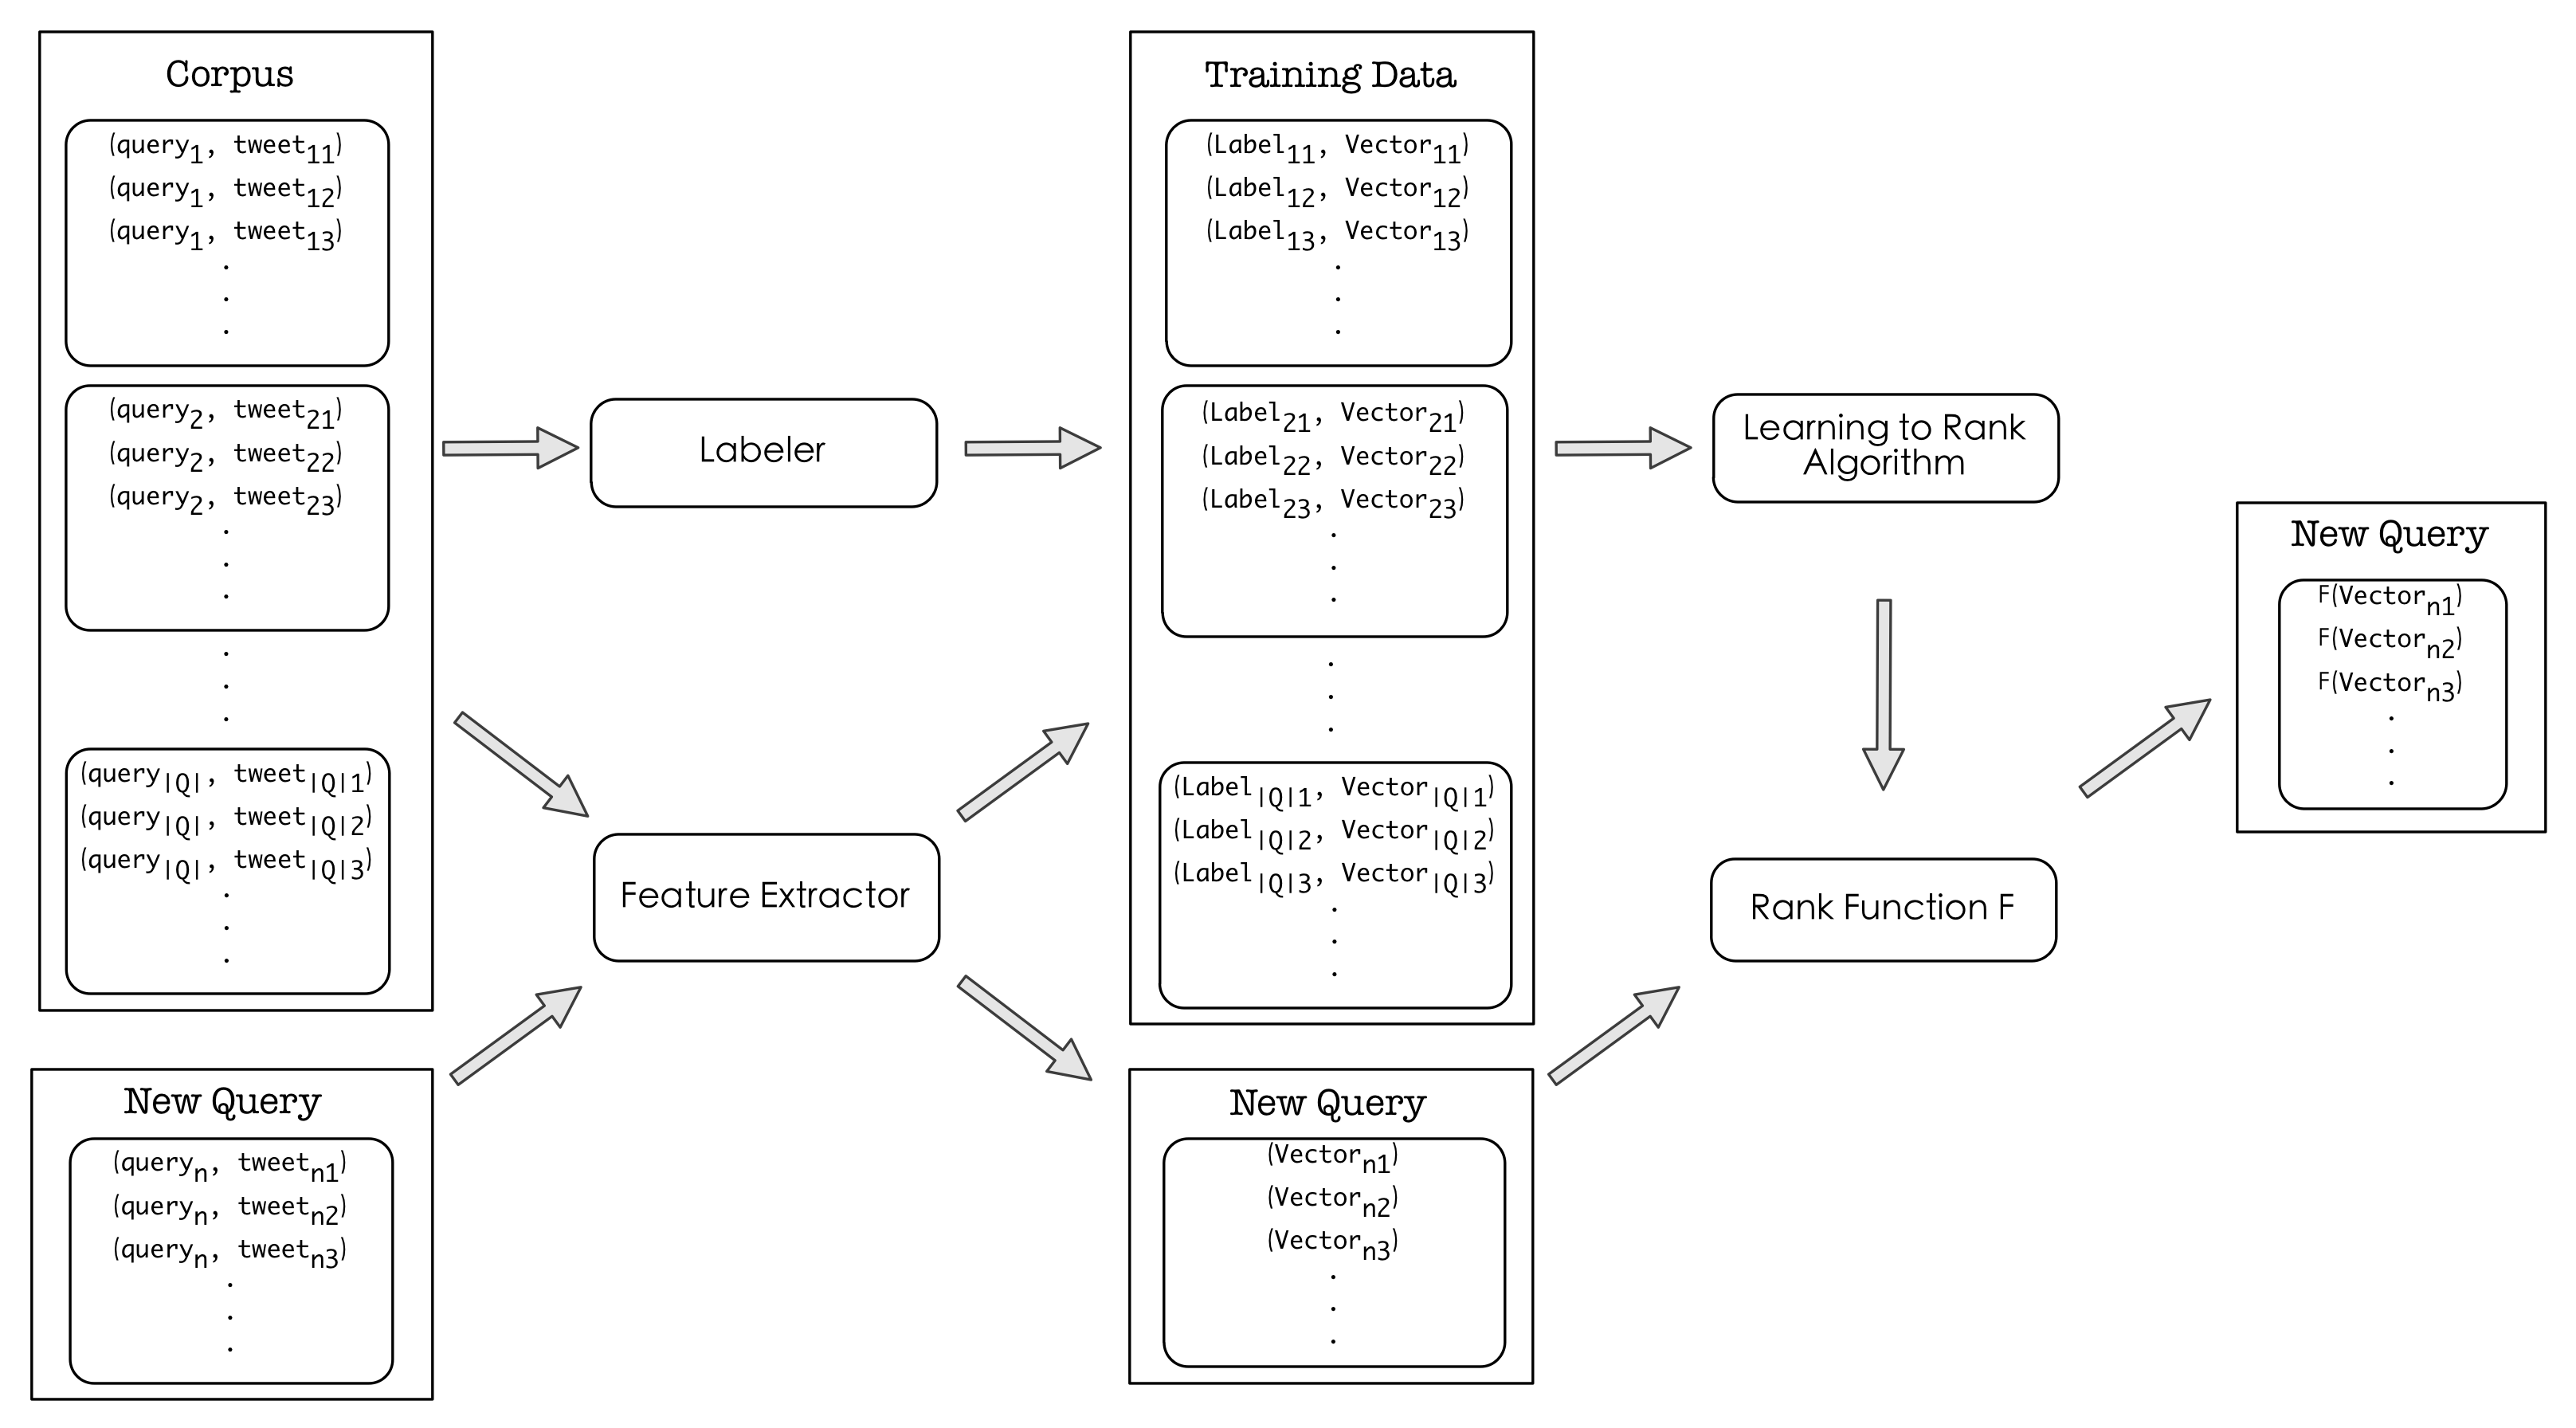
\includegraphics [width=600pt]{Framwork.png}
\caption{Twitter检索排序学习框架}
\label{Framework}
\end{figure*}
\end{landscape}
另外,对于有监督学习来说,一个重要的条件就是大量的训练数据,但是在排序学习过程中,大量人工标注训练数据是不现实的,但是搜索引擎可以通过用户的点击动作模拟点击网页与用户查询的相关性,以此获得大量的训练数据。

 对于Twitter中的信息检索,我们可以通过排序学习模型对给定关键词的tweet集合进行排序。我们的目的是验证我们开发的特征是否对于Twitter的排序有效,因此使用不同特征集合排序模型在Twitter中tweet排序结果可以反映不同特征的有效性。图~\ref{Framework}给出了基于排序学习的Twitter检索框架。
 

首先给定一个查询集合$Q$及其对应的tweet作为训练集,每个$tweet_{ij}$被手工标注了是否与对应的查询词$query_i$相关。一系列与tweet查询相关的特征被设计和开发,形成特征向量 $Vector_{ij}$。接着,应用排序学习算法对手工标注的数据进行训练生成排序学习模型。对于一个新的查询和其所对应的tweet,抽取相同的特征形成特征向量$Vector$,然后利用生成好的排序学习模型对tweet进行相关排序。对特定一组特征生成的排序模型在测试数据集上的排序表现能够反映特征对于排序任务的有效性。

这里要强调的是,本文所涉及的Twitter检索、Twitter观点检索、Twitter传播观点发现和Twitter传播者发现任务都采用了排序学习框架,通过不同特征组合形成的模型,在排序效果上的表现,说明Twitter中哪些tweet文本特征和Twitter的社交媒体特征会影响对应的任务。



 \subsection{Twitter积木特征}
 对于每一个tweet,我们从Twitter积木及其结构中设计了一系列特征,并称之为Twitter积木特征(TBB features)。这些Twitter积木特征仅仅利用了tweet的文本信息并未利用其他社交媒体属性。我们将这些特征分为如下几个类别:
 
 \begin{figure}[htp]
\centering
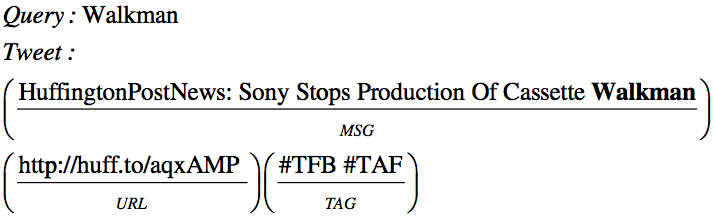
\includegraphics[height=100pt]{TBB_fea.png}
\caption{一个查询词和一个tweet}
\label{TBB_fea}
\end{figure}

 \begin{enumerate}
\item {\bf Twitter积木结构类型(TBB Structure Type)}:每个tweet都有自身不同的结构。我们设计了一个15维的特征向量,其中特征向量中的每个维度表示当前tweet是否是特定的某种Twitter积木结构。我们选取14种经常使用的Twitter积木结构作为特征维度,其他很少使用的Twitter积木结构作为剩下的特征维度(见表~\ref{TBB_Distr})。如果tweet是某个Twitter积木结构,则特征向量中所对应的特征维为1,其他特征维为0。例如,图~\ref{TBB_fea}中tweet的Twitter积木结构是“MSG URL TAG”,则特征向量所对应的该维特征取值为1,其他维取值为0。
\item {\bf 查询词Twitter积木位置(TBB Query Position)}:我们利用六个维度的特征向量表示查询词所在Twitter积木的位置。因为一个查询词经常是一个短语或是一个hashtag,所以特征表示为查询词是否在普通文本积木(MSG)、观点积木(COM)、标签积木(TAG)的开头或中间。例如,图~\ref{TBB_fea}中查询词“Walkman”就在普通文本积木(MSG)中间。如果查询词在对应的积木位置,则特征值为1,否则为0。
\item {\bf 邻近Twitter积木类型(Neighbour TBB Type)}:查询词所在Twitter积木的前后积木类型同样具有重要的信息,我们将其利用与开发。特征包括查询词所在Twitter积木的前后积木是否是标签积木(TAG)、提及积木(MET)、转发积木(RWT)、链接积木(URL)、普通文本积木(MSG)、观点积木(COM)。例如,图~\ref{TBB_fea}中查询词“Walkman”所在积木的后个积木是链接积木(URL)。
\item {\bf Twitter积木数目(TBBs Count)}:直觉上如果一个tweet存在较多的包含查询词的Twitter积木,则该tweet更有可能是人们需要的相关tweet。因此,我们设计了一个特征,这个特征表示tweet中存在几个包含查询词的Twitter积木。例如,图~\ref{TBB_fea}中tweet中仅仅存在一个包含“Walkman”查询词的Twitter积木。
\item {\bf Twitter积木长度(TBB Length)}:直觉上如果tweet中包含查询词的Twitter积木长度越长,则该tweet中与查询词相关的信息则越多。因此,我们设计了最长包含查询词Twitter积木词个数的特征。
\item {\bf Twitter积木OOV值(TBBs OOV)}:这个特征计算tweet中存在未登录词的比例,以此评估Twitter积木的质量。
\item {\bf Twitter积木语言(TBB Language)}:这是一个布尔特征用来表示包含查询词的Twitter积木是否是英语,因为人们一般会选择语言是母语的tweet作为相关tweet。
 \end{enumerate} 
 
\section{Twitter信息检索实验}
 \subsection{Twitter信息检索实验数据}
 我们利用Twitter streaming API每天获取80万个tweet并建立索引,然后构造了一个搜索引擎。三个用户参与实验并标注数据,这三个用户都是计算机科学研究人员,它们从2010年10月4日至2010年10月28日使用我们的搜索引擎。它们任意输入自己喜欢的查询词,然后搜索引擎根据BM25算法\footnote{BM25具体算法将在~\ref{Baseline}介绍。}对收集的tweet进行排序并返回结果,搜索引擎默认返回10个tweet,另外,返回的tweet中同时显示时间信息和tweet的作者信息。然后这三个用户根据返回tweet是否与查询词相关对tweet进行标注,如果相关则标为1,否则为0。最后我们总共收集了100个查询词和其返回的tweet。我们对这100个查询词及其tweet进行分析与统计,发现这100个tweet大致可以分成六类(见表~\ref{Data_aaai_cata})。这六类中数目最多的是“热点”类,如:查询词“Chilean miner”,另外,还有很大一部分查询词与科技相关(归为“科技”类),如查询词“java flaw”,“新闻”类是一些重要的新闻信息,如“wikileaks”,有意思的是三个用户还输入了一些“地理”查询词,以此期望在Twitter中找到一些所在地的信息,“娱乐”类中包含了一些电影和明星的查询词,剩下的查询词都归为“其他”类。

 \begin{table}[htp]
\centering
\caption{Twitter信息检索查询词类别及其数目}
\label{Data_aaai_cata}
 \begin{tabular}{|l |c|}
 \hline
\textbf{类别}& \textbf{数目 }\\ 
 \hline
 热点 & 34 \\ 
科技 & 27 \\
新闻 & 17 \\
地理 & 8 \\
娱乐 & 8 \\
其他 & 6 \\
 \hline
\end{tabular}
\end{table}

表~\ref{Data_aaai_stat}则给出了实验数据的一些统计信息。

 \begin{table}[htp]
\centering
\caption{Twitter信息检索实验数据统计信息}
\label{Data_aaai_stat}
 \begin{tabular}{|l r|}
 \hline
查询词长度(词数)& 1.48 \\
查询词对应tweet平均数目 & 9.36 \\
相关tweet总数目 & 184 \\
非相关tweet总数目 & 752 \\
 \hline
\end{tabular}
\end{table}

\subsection{信息检索评价指标}
\label{MAP}
平均准确率(Mean Average Precision-MAP)是信息检索中经常使用的评价指标\upcite{voorhees1999natural,voorhees2000variations}。它对相关文档与不相关文档的排序非常敏感。我们利用平均准确率来评价排序系统的有效性。计算平均准确率的公式如下:
$$MAP(Q)=\frac{1}{|Q|}\sum_{q=1}^{|Q|}AveP(q)$$
其中$Q$是查询词集合,$|Q|$ 是查询词集合中查询词数目,$AveP(q)$是查询词$q$的平均准确率。
$$AveP(q)=\frac{1}{|rel|}\sum_{n:p_n = 1}Prec@n$$
其中$|rel|$是相关文档数目,$Prec@n$ 是检索到 top $n$个文档中相关文档的比例。
$$Prec@n=\frac{|{i:1\leq i \leq n,p_i =1}|}{n}$$
其中$p_i = 1$表示排在第$i$个位置的文档是相关文档。

\subsection{Twitter信息检索实验设置和基准系统(Baseline)}
我们进行了10次交叉验证,并将Duan等人的方法作为我们的基准系统(Baseline)\upcite{duan2010empirical},这个系统目前是最好的基于排序学习的Twitter信息检索系统。基准系统在我们构造的数据集上tweet的排序平均准确率为0.344。我们没有采用Duan等人使用的以BM25分值作为排序基础的基准系统,因为我们的系统和Duan等人的系统在排序效果上都显著好于BM25系统。另外,我们还开发了一个利用社交媒体特征的Twitter信息检索系统,称之为 SM\_Rank。表\ref{Baseline_aaai_fea}列出了Baseline和Social Media两个系统所使用的特征。我们将利用Twitter积木标注器自动标注积木然后抽取结构化特征开发的Twitter信息检索系统称为TBB\_Rank。最后基于三组不同特征集合组合的系统分别称为 Baseline+SM\_Rank, Baseline+TBB\_Rank, SM+TBB\_Rank。

\begin{table}[htp]
 \centering
 \caption{基准系统特征(Baseline Features)和 社交媒体特征(Social Media Features)}
 \label{Baseline_aaai_fea}
 \begin{threeparttable}
 \begin{tabular}{|lp{3.0in}|}
\hline
\textbf{基准系统特征(Baseline Features)} & \textbf{描述} \\
 \hline
链接(Link) & tweet中是否包含链接\\
长度(Length) & tweet中包含的词数目 \\
重要粉丝(Important\_follower)& tweet的作者或转发该tweet的用户中follower score\tnote{1}最高的用户粉丝数目\\ 
提及总和(Sum\_mention) & tweet的作者和转发该tweet的用户mention scores~\tnote{2}的总和\\ 
分组数目(First\_list) &  tweet的作者List score\tnote{3}\\ 
 \hline 
 \hline 
\textbf{ 社交媒体特征(Social Media Features)} & \textbf{描述} \\
 \hline
粉丝数目(Followers) &  tweet的作者的粉丝数目 \\
朋友数目(Friends) & tweet的作者的朋友数目 \\
分组数目(Listed) & tweet的作者的分组数目 \\
提及(Mentions)& tweet是否包含提及 \\
Hashtag数目(Hashtags) & tweet中包含hashtag的数目 \\  
回复(Reply) & tweet是否是回复 \\
转发(Retweeted) & tweet是否是转发 \\
来源(Source Web) & tweet的消息是否来源于web \\
发布数目(Statuses ) &   tweet的作者以往发布tweet的数目 \\  
转发数目(Retweet Count)& tweet被转发的次数 \\ 
作者被转发数目(Author Retweet Count )& tweet的作者在收集的tweet中被转发的次数 \\  
公共词数目(Overlap Words) & 查询词与tweet公共词数目 (Jaccard score) \\  
Tweet发布时间(Recency)& tweet发布时间到用户输入查询词的时间差 (以秒计)\\   
 \hline
 \end{tabular}
 \begin{tablenotes}
        \footnotesize
\item[1] Follower Score:用户粉丝数目;
\item[2] Mention Score:在收集的tweet中用户被提及的个数;
\item[3] List Score: 用户的分组数目。
\end{tablenotes}
    \end{threeparttable}
\end{table}

 \subsection{Twitter信息检索实验结果及分析}
 
表~\ref{Res_aaai_TBB}给出了各个Twitter信息检索系统的tweet排序实验结果。我们可以看到仅仅从tweet文本获取结构化信息构造的TBB\_Rank系统,在排序效果上可以达到与Baseline和SM\_Rank系统相当的效果。我们进行了显著性测试(paired t-test),发现三个系统在实验结果上没有显著性差异($p=0.05$)。我们进一步发现将Twitter积木特征和社交媒体特征结合使用的SM+TBB\_Rank系统能够显著提高tweet排序效果。最后将三组特征集合一起使用的Baseline+SM+TBB\_Rank系统获得最高平均准确率0.4712。所有这些都说明结构化信息能够帮助Twitter信息检索。

\begin{table}[htp]
 \centering
 \caption{基于排序学习的Twitter信息检索实验结果}
  \label{Res_aaai_TBB}
 \begin{tabular}{|l | l|}
 \hline
 & \textbf{MAP} \\
 \hline
 Baseline & 0.4197 \\
 SM\_Rank & 0.4338 \\
 TBB\_Rank & 0.4235 \\
 Baseline+SM\_Rank & 0.4546 \\
 Baseline+TBB\_Rank & 0.4326 \\
 SM+TBB\_Rank & 0.4710$^{\ast\dagger}$\\
 Baseline+SM+TBB\_Rank & 0.4712$^{\ast\dagger}$\\
 \hline
 \end{tabular}
  \begin{tablenotes}
        \footnotesize
\item $^{\ast}$和$^{\dagger}$分别表示排序结果显著高于Baseline和SM\_RankTwitter信息检索系统。
\end{tablenotes}
\end{table}

Duan等人发现一个tweet中是否包含一个链接是基于排序学习的Twitter信息检索系统中最重要的特征\upcite{duan2010empirical}。我们在此基础上进一步研究分析了那种包含链接积木(URL)的Twitter积木结构对于tweet排序更加重要。我们将问题转化为表~\ref{URL_aaai_fea}中的特征那个对于tweet排序更加重要。我们将这些特征一个一个替换基准系统中的链接(Link)特征,然后观察平均准确率的变化。

\begin{table}[htp]
 \centering
 \caption{基于链接积木(URL)的Twitter积木结构特征}
 \label{URL_aaai_fea}
 \begin{tabular}{|lp{4.0in}|}
 \hline
 \textbf{链接积木(URL)特征} & \textbf{描述} \\
 \hline
MSG URL & tweet的Twitter积木结构是否是“MSG URL” \\     
RWT MSG URL&  tweet的Twitter积木结构是否是“RWT MSG URL” \\     
COM URL &  tweet的Twitter积木结构是否是“COM URL”\\     
TAG MSG URL&  tweet的Twitter积木结构是否是“TAG MSG URL” \\      
RWT MSG URL &  tweet的Twitter积木结构是否是“RWT MSG URL”\\                      
MSG URL TAG &  tweet的Twitter积木结构是否是“MSG URL TAG”\\    
OTHER URL &  tweet的Twitter积木结构是否是其他包含链接积木(URL)的非常用积木结构\\               
 \hline
 \end{tabular}
\end{table}

表~\ref{Res_aaai_TBB_URL}给出了实验结果。我们发现特征“MSG URL”能够在基准系统中(Baseline)替换链接(Link)特征时,平均准确率没有显著下降($p=0.05$),而其他特征的替换都显著地影响了系统的tweet排序效果,这说明这个特征能够取代基准系统中(Baseline)的链接(Link)特征,同时也说明了一个tweet的Twitter积木结构是否是“MSG URL”对于tweet排序具有重要的影响。这个原因可能是因为大多数包含链接tweet的Twitter积木结构是“MSG URL”(见表~\ref{TBB_Distr}),而如果一个tweet它的结构是“MSG URL”则它很有可能是相关tweet。例如在我们的实验数据中存在如下例子,查询词为“wikileaks”,它有两个对应的tweet:

\begin{description}
\item{(a)} \emph{Obama administration braces for WikiLeaks release of thousands
	of secret documents on Iraq war (Star Tribune) \url{http://bit.ly/9lnBGB}}

\item{(b)} \emph{BBCWorld: Wikileaks files 'threaten troops'
	\url{http://bbc.in/c4Sznk}: BBCWorld: Wikileaks files 'threaten troops'...
	\url{http://dlvr.it/7P7zM}}
\end{description}

标注者将 Tweet (a)标注为相关tweet而 Tweet (b)标注为不相关tweet。 Tweet (a)的Twitter积木结构是“MSG URL", Tweet (b)的Twitter积木结构是“MSG URL MSG URL"。标注Tweet (b)为不相关tweet的原因可能是这个tweet包含两个链接积木(URL),造成读者理解这个tweet比较混乱。在我们的实验中,我们的基准系统(Baseline)和SM\_Rank系统都将Tweet (b)排在Tweet (a)前面,而TBB\_Rank 系统则将Tweet (a)排在Tweet (b)前面。这说明我们的Twitter积木能够获取更多的包含链接tweet的信息,并以此改善tweet的排序效果。

\begin{table}[htp]
 \centering
 \caption{基于链接积木(URL)的Twitter积木结构特征排序实验结果}
 \label{Res_aaai_TBB_URL}
 \begin{tabular}{|l | r|}
 \hline
 & \textbf{MAP} \\
 \hline
Baseline & 0.4197 \\
MSG URL & 0.4019 \\
MSG URL TAG & 0.3327\\
RWT MSG URL& 0.3289 \\
TAG MSG URL& 0.3245 \\
COM URL & 0.3191 \\
OTHER URL & 0.1984\\
MET MSG URL & 0.1932\\
 \hline
 \end{tabular}
\end{table}

\vspace{0.5cm}

\section{小结}
本章我们介绍了Twitter积木及其结构的定义与识别,并以此获取tweet的结构化信息。我们分析了不同Twitter积木结构具有不同属性,例如,不同Twitter积木结构所对应tweet的OOV值明显不同。我们基于Twitter积木及其结构设计了一系列特征,并将其利用到基于排序学习的Twitter信息检索应用中,实验结果表明,在tweet排序上仅仅使用我们设计的结构化特征,能够达到当今最好的基于排序学习的Twitter信息检索系统的效果。如果将社交媒体特征和结构化特征结合使用能够得到更好的tweet排序效果。以上工作说明虽然tweet文本十分简短,但是其文本依然具有结构化信息,并能够帮助提高Twitter信息检索的效果。
